\section{Output}

Intro text required



\subsection{HDMI}

HDMI is a two-way communication protocol and supports many different formats/frequencies/specs. Many monitors/recorders only support a subset of these formats and expect signals to conform to certain values. These values are not documented publicly so we are currently in the process of debugging device compatibility one by one. The good thing is that it's a pure software thing and we can add support and test compatibility with additional devices as time progresses.\\

In general we discovered that monitors are more flexible when it comes to HDMI (TMDS) freqencies as they just "tune" into (sync to) the provided clock/data rate. Recorders expect signals to be in a much stricter/narrower range and will not work (show "no signal") if there is a minor deviation. 

Watch this 33C3 talk by Tim Ansell about \href{https://media.ccc.de/v/33c3-8057-dissecting_hdmi}Dissecting HDMI} to get insight into how HDMI works.


\subsubsection{External HDMI Recording}

Settings for VSync, HSync, etc. inside the AXIOM Beta can be found in: 

\consoleCommand{/root/gen\_init.sh}

For example the Atomos SHOGUN was found to work with these HDMI parameters: 

\consoleCommand{    scn_reg  0 2200             # total_w
    scn\_reg  1 1125             # total_h
    scn\_reg  2   60             # total_f
     
    scn\_reg  4  262             # hdisp\_s
    scn\_reg  5 2182             # hdisp\_e
    scn\_reg  6   45             # vdisp\_s
    scn\_reg  7 1125             # vdisp\_e
     
    scn\_reg  8    0             # hsync\_s
    scn\_reg  9 2100             # hsync\_e
    scn\_reg 10    4             # vsync\_s
    scn\_reg 11    9             # vsync\_e
     
    scn\_reg 32  252             # pream\_s
    scn\_reg 33  260             # guard\_s
    scn\_reg 34  294             # terc4\_e
    scn\_reg 35  296             # guard\_e}

Currently it is not possible to alter TMDS and Clock frequencies from the userspace (requires new FPGA bitstream).\\

For the firmware there are two modes available, the 30Hz and 60Hz variant. You can switch between them quite easily.\\

cmv\_hdmi3.bit is the FPGA bitstream loaded for the HDMI interface. We use symlinks to switch this file easily.\\

Before doing this, don't forget to check if the files (cmv\_hdmi3_60.bit or cmv\_hdmi3_30.bit) really exist in the /root folder.\\

The output is always in 8bpc RGB color space without subsampling (4:4:4). Not all capture devices can manage this.\\

Other modes like YCrCb, etc. are currently not supported.\\ 



\paragraph{Devices Confirmed Working}

Atomos Shogun - AXIOM Beta supports up to 1080p60 
Atomos Ninja - AXIOM Beta supports up to 1080p30
Blackmagic Video Assist and Video Assist 4K - AXIOM Beta supports up to 1080p60\\

\textbf{Blackmagic Video Assist and Video Assist 4K}

\begin{center}
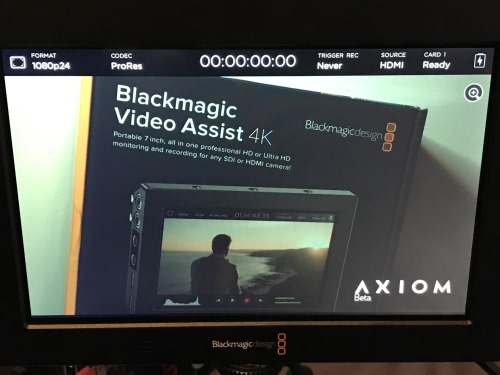
\includegraphics[height=8cm]{images/AxiomBetaBMVA4K}\\
\end{center}
 
Changes for Blackmagic Video Assist and Video Assist 4K, tested on firmware 2.3.1:\\

\textbf{edit setup.sh}\\

Add: 

\consoleCommand{./gen\_init.sh 1080p60BMVA}

comment out any other ./gen\_init.sh entries. 

\textbf{edit gen\_init.sh}

\consoleCommand{./gen\_init.sh 1080p60BMVA}

\textbf{edit gen\_init.sh}

Replace:

\consoleCommand{SHOGUN)}

With:

\consoleCommand{SHOGUN|1080p60BMVA|1080p30BMVA)}

Add the section below:

\consoleCommand{  1080p50BMVA|1080p25BMVA)
    scn\_reg  0 2640             # total\_w
    scn\_reg  1 1125             # total\_h
    scn\_reg  2   60             # total\_f
 
    scn\_reg  4  262             # hdisp\_s
    scn\_reg  5 2182             # hdisp\_e
    scn\_reg  6   45             # vdisp\_s
    scn\_reg  7 1125             # vdisp\_e
 
    scn\_reg  8    0             # hsync\_s
    scn\_reg  9 2100             # hsync\_e
    scn\_reg 10    4             # vsync\_s
    scn\_reg 11    9             # vsync\_e
 
    scn\_reg 32  252             # pream\_s
    scn\_reg 33  260             # guard\_s
    scn\_reg 34  294             # terc4\_e
    scn\_reg 35  296             # guard\_e
    ;;
    
      1080p24BMVA)
    scn\_reg  0 2750             # total\_w
    scn\_reg  1 1125             # total\_h
    scn\_reg  2   60             # total\_f
 
    scn\_reg  4  262             # hdisp\_s
    scn\_reg  5 2182             # hdisp\_e
    scn\_reg  6   45             # vdisp\_s
    scn\_reg  7 1125             # vdisp\_e
 
    scn\_reg  8    0             # hsync\_s
    scn\_reg  9 2100             # hsync\_e
    scn\_reg 10    4             # vsync\_s
    scn\_reg 11    9             # vsync\_e
 
    scn\_reg 32  252             # pream\_s
    scn\_reg 33  260             # guard\_s
    scn\_reg 34  294             # terc4\_e
    scn\_reg 35  296             # guard\_e
    ;;
    
    }


\subsubsection{Experimental UHD Raw Recording}

\textbf{Note:} This experimental raw mode works only in 1080p60 (A+B Frames) and is only tested with the Atomos Shogun currently. \\

To measure the required compensations with a different recorder see \textbf{Raw processing recorder benchmarking}\\

This mode requires darkframes which are created in the course of a camera Factory Calibration. Early Betas are not calibrated yet - this step needs to be completed by the user. See \textbf{Factory Calibration}.\\

\paragraph{Enable raw recording mode}\\

Input:

\consoleCommand{./hdmi\_rectest.sh}

Inside that script the following command is worth noting:\\

Enable experimental raw mode: 

\consoleCommand{scn\_reg 31 0x0A01}

Disable experimental raw mode: 

\consoleCommand{scn\_reg 31 0x0001}

If you get an error report like this: 

\consoleCommand{    Traceback (most recent call last):
      File "rcn_darkframe.py", line 17, in <module>
        import png
    ImportError: No module named 'png'}
    
Make sure the Beta is connected to the Internet via Ethernet and run:     

\consoleCommand{pip install pypng}



\paragraph{Processing}

Postprocessing software to recover the raw information (DNG sequences) is on github in \href{https://github.com/apertus-open-source-cinema/misc-tools-utilities/tree/master/raw-via-hdmi}{RAW via HDMI}\\

Required packages: ffmpeg build-essentials

Mac requirements for compiling: gcc4.9(via homebrew): 

\consoleCommand{brew install homebrew/versions/gcc49}

Also install ffmpeg

To do all the raw processing in one single command (after ffmpeg codec copy processing): 

\consoleCommand{./hdmi4k INPUT.MOV - | ./raw2dng --fixrnt --pgm --black=120 frame%05d.dng}

\subsubsection{EDL Parser}
\subsubsection{cmv perf3}
\subsection{SDI}
\subsection{Modes}



\subsection{Generator and HDMI Output}
\subsection{Stopping and Starting HDMI Live-stream}

Stop HDMI live stream: 

\consoleCommand{fil\_reg 15 0} 

Start HDMI live stream: 

\consoleCommand{fil\_reg 15 0x01000100} 